\documentclass[a4paper,12pt]{article}
\usepackage[russian]{babel}
\usepackage[T2A]{fontenc}
\usepackage[utf8]{inputenc}
\usepackage{geometry}
\usepackage{amsmath}
\usepackage{graphicx}
\usepackage{cancel}
\usepackage{float} 
\usepackage{xcolor}
\usepackage{array}
\usepackage{caption}
\usepackage{booktabs}
\usepackage{amssymb}
\usepackage{subcaption}
\usepackage{pgfplots}
\pgfplotsset{compat=1.18}
\usetikzlibrary{arrows.meta, matrix}
\usepackage{capt-of}
\usepackage{multirow}
\usepackage[siunitx]{circuitikz}
\usepackage[bottom]{footmisc}
\usepackage{tcolorbox}
\usepackage{nicematrix}
\usepackage{tikz}
\usetikzlibrary{positioning, arrows.meta}

% --- hyperref ОДИН РАЗ ---
\usepackage{hyperref}
\hypersetup{linktoc=page}
\hypersetup{
	colorlinks=true,
	linkcolor=red,
	citecolor=red,
	urlcolor=red,
	filecolor=red,
}

% --- Содержание ---
\usepackage{tocloft}
\usepackage{etoolbox}
\usepackage{hyperref}
\hypersetup{
	colorlinks=true,
	linkcolor=red,
	citecolor=red,
	urlcolor=red,
}

% Патчим \tableofcontents: текст строк — без ссылок и чёрный
% Это делается через замену \contentsline внутри TOC
\preto\tableofcontents{%
	\begingroup
	% Переопределяем contentsline так, чтобы текст был чёрным без ссылки,
	% а номер страницы — красной ссылкой
	\renewcommand{\contentsline}[4]{%
		\ifnum\pdfstrcmp{##1}{section}=0
		\vskip 4pt{\normalfont\color{black}##2}\nobreak\hfill
		{\normalfont\color{red}\hyperlink{##4}{##3}}\par
		\else\ifnum\pdfstrcmp{##1}{subsection}=0
		\vskip 2pt\hspace{1.5em}{\normalfont\color{black}##2}\nobreak\hfill
		{\normalfont\color{red}\hyperlink{##4}{##3}}\par
		\else
		\vskip 1pt\hspace{3em}{\normalfont\color{black}##2}\nobreak\hfill
		{\normalfont\color{red}\hyperlink{##4}{##3}}\par
		\fi\fi
	}%
}
\appto\tableofcontents{\endgroup}

% tocloft — только для отступов, без переопределения шрифтов
\usepackage{tocloft}

% --- Листинги ---
\usepackage{listings}

\definecolor{codebg}{RGB}{250,250,252}
\definecolor{linenumcolor}{RGB}{150,150,170}
\definecolor{mathblue}{RGB}{30,100,200}
\definecolor{mathorange}{RGB}{200,100,20}
\definecolor{matlabblue}{RGB}{0,0,200}
\definecolor{matlabgreen}{RGB}{30,130,30}
\definecolor{matlaborange}{RGB}{200,80,0}


\lstdefinestyle{matlab}{
	language=Matlab,
	basicstyle=\ttfamily\small,
	keywordstyle=\color{matlabblue}\bfseries,
	commentstyle=\color{matlabgreen}\itshape,
	stringstyle=\color{matlaborange},
	numberstyle=\tiny\color{linenumcolor},
	numbers=left,
	numbersep=10pt,
	backgroundcolor=\color{codebg},
	frame=single,
	frameround=tttt,
	framesep=4pt,
	rulecolor=\color{matlabblue!30},
	breaklines=true,
	tabsize=4,
	showstringspaces=false,
	captionpos=b,
	xleftmargin=15pt,
	xrightmargin=5pt,
	escapeinside={\%*}{*)},
	morekeywords={cvx_begin,cvx_end,sdp,variable,minimize,maximize},
}

\lstset{style=matlab}

\renewcommand{\lstlistingname}{Листинг}
\DeclareCaptionFormat{redlisting}{#1\textcolor{red}{#2}#3}
\captionsetup[lstlisting]{format=redlisting}

\geometry{left=1.5cm, right=2cm, bottom=2cm, top=2cm}
\captionsetup[figure]{name=Рисунок}
\captionsetup[table]{name=Таблица}
\captionsetup{labelsep=endash}

\newcommand{\figwidth}{0.65\textwidth}

\begin{document}
	
	\begin{titlepage}
		\centering
		
		\vspace*{0.5cm}
		{\small
			Министерство науки и высшего образования Российской Федерации\\[2pt]
			Федеральное государственное автономное образовательное учреждение\\
			высшего образования\\[2pt]
			\textbf{«Национальный исследовательский университет ИТМО»}\\
		}
		
		\vspace{0.8cm}
		\hrule height 0.8pt
		\vspace{0.3cm}
		
		{\large Факультет систем управления и робототехники}
		
		\vspace{0.3cm}
		\hrule height 0.4pt
		\vspace{2.5cm}
		
		{\Huge\bfseries ОТЧЁТ}\\[0.4cm]
		{\LARGE\bfseries о лабораторной работе}\\[0.8cm]
		
		\begin{tcolorbox}[
			colback=gray!4,
			colframe=gray!10,
			boxrule=0.8pt,
			arc=4pt,
			left=12pt, right=12pt, top=8pt, bottom=8pt
			]
			\centering
			{\large По дисциплине:\\[4pt]}
			{\large\bfseries «Теория автоматического управления»}\\[10pt]
			{\large Тема:\\[4pt]}
			{\large\bfseries «Слежение и компенсация. Франкис, Дэвисон и наблюдатели.»} \\[10pt]
			{\large Поток: 1.1.3 \( \) Вариант: 25}
		\end{tcolorbox}
		
		\vspace{3cm}
		
		\begin{minipage}{0.45\textwidth}
			\raggedright
			{\large\bfseries Студент:}\\[4pt]
			Охрименко Е.\,Д.\\
		\end{minipage}
		\hfill
		\begin{minipage}{0.45\textwidth}
			\raggedleft
			{\large\bfseries Преподаватель:}\\[4pt]
			Пашенко А.\,В.\\
		\end{minipage}
		
		\vfill
		\vspace{0.4cm}
		{\large Санкт-Петербург, 2026}
	\end{titlepage}
	
	\newpage
	\tableofcontents
	
	\newpage \section{Синтез регуляторов при помощи матричных уравнений Франкиса-Дэвисона}\label{sec:1}
	
	В соответствии с вариантом рассмотрю систему:
	
\begin{equation}
	\begin{cases}
		\dot{x} = Ax + Bu + B_f f \\
		y = Cx + Du + D_f f
	\end{cases}
	\qquad
	x(0) = \begin{bmatrix} 0 & 0 & 0 \end{bmatrix}^T
		\label{sys}
\end{equation}
	
	где:
	
	\[
	A = \begin{bmatrix} 
		8 & 1 & 11 \\ 
		4 & 0 & 4 \\ 
		-4 & -3 & -7 
	\end{bmatrix} \quad
	B = \begin{bmatrix} -1 \\ -3 \\ 3 \end{bmatrix} \quad
	B_f = \begin{bmatrix} 
		1 & -1 \\ 
		0 & 0 \\ 
		-1 & 0
	\end{bmatrix}
	\]
	
	\[
	C = \begin{bmatrix} -2 & 0 & -3 \end{bmatrix} \quad
	D = 15 \quad
	D_f = \begin{bmatrix} 0 & 3 \end{bmatrix}
	\]
	
	Генератор внешнего возмущения:
	
\begin{equation}
	\begin{cases}
		\dot{w}_f = \Gamma_f w_f \\
		f = Y_f w_f
	\end{cases}
	\qquad
	w_f(0) = \begin{bmatrix} 1 & 1 & 1 & 1 \end{bmatrix}^T
		\label{genF}
\end{equation}
	
	где:
	
	\[
	\Gamma_f = \begin{bmatrix}
		35 & 10 & -28 & 17 \\
		-22 & -7 & 18 & -12 \\
		56 & 17 & -45 & 27 \\
		34 & 12 & -28 & 17
	\end{bmatrix} \quad
	Y_f = \begin{bmatrix}
		-6 & -2 & 4 & -3 \\
		12 & 4 & -10 & 6
	\end{bmatrix}
	\]
	
	Генератор задающего воздействия:
	
	\begin{equation}
		\begin{cases}
			\dot{w}_g = \Gamma_g w_g \\
			g = Y_g w_g
		\end{cases}
		\qquad
		w_g(0)
		\label{gen}
	\end{equation}
	
	где:
	
	\begin{equation}
		g(t) = 21\sin(2t) - 12
		\label{g}
	\end{equation}
	
	Требуется:
	\begin{enumerate}
		\item Найти собственные числа матрицы $\Gamma_f$, определить моды внешнего возмущения и их характер.
		
		\item Определить матрицы $\Gamma_g$, $Y_g$ и начальное условие $w_g(0)$, при которых генератор порождает $g(t)$. Найти $\sigma(\Gamma_g)$.
		
		\item Построить схему моделирования системы, замкнутой регулятором $u = Kx + K_g w_g + K_f w_f$, обеспечивающим $\lim\limits_{t\to\infty} |g(t) - y(t)| = 0$.
		
		\item Синтезировать ``feedback''-компоненту $K$ любым пройденным способом. Привести выкладки и матрицу $K$.
		
		\item Составить и проверить разрешимость матричных уравнений Франкиса–Дэвисона для $K_g$. Синтезировать $K_g$.
		
		\item Составить и проверить разрешимость уравнений Франкиса–Дэвисона для $K_f$. Синтезировать $K_f$.
		
		\item Выполнить компьютерное моделирование для 5 режимов ($u=0$, $u=Kx$, $u=Kx+K_f w_f$, $u=Kx+K_g w_g$, полный регулятор) и построить графики $f(t), g(t), u(t), x(t), y(t), e(t)$.
		
		\item Проанализировать полученные результаты и сделать выводы.
	\end{enumerate}
	
	\hrule \newpage
	
	\subsection{Анализ матрицы \(\Gamma_f\)}
	
	Для начала найду собственные числа матрицы \(\Gamma_f\), (листинг~\ref{lst:eig1}):
	
	\[
	\sigma(\Gamma_f) = \{\pm 3\mathrm{j},\; \pm \mathrm{j}\}
	\]
	
	
	Собственные числа матрицы \(\Gamma_f\) являются чисто мнимыми и попарно сопряженными. Внешнее возмущение \(f(t)\) --- сумма гармонических колебаний с частотами 3 и 1.
	
	\subsection{Синтез генератора задающего воздействия}
	
	Для генерации сигнала \eqref{g} использую систему \eqref{gen}. 
	Её решение:
	\[
	w_g(t) = e^{\Gamma_g t} w_g(0), \quad
	g(t) = Y_g w_g(t) = Y_g e^{\Gamma_g t} w_g(0)
	\]
	
	Сигнал \(g(t) = 21\sin(2t) - 12\) содержит постоянную составляющую (\(-12\)) и гармонику с частотой \(\omega = 2\) и амплитудой \(21\). Для его генерации необходимы моды:
	\[
	\lambda_1 = 0 \quad \lambda_{2,3} = \pm 2i
	\]
	
	Выбираю матрицу динамики:
	\[
	\Gamma_g =
	\begin{bmatrix}
		0 & 0 & 0 \\
		0 & 0 & 2 \\
		0 & -2 & 0
	\end{bmatrix} \quad
	e^{\Gamma_g t} =
	\begin{bmatrix}
		1 & 0 & 0 \\
		0 & \cos(2t) & \sin(2t) \\
		0 & -\sin(2t) & \cos(2t)
	\end{bmatrix}
	\]
	
	Ввожу состояние генератора:
	\[
	w_g(t) =
	\begin{bmatrix}
		w_1(t) \\ w_2(t) \\ w_3(t)
	\end{bmatrix} \quad
	w_g(0) =
	\begin{bmatrix}
		w_1(0) \\ w_2(0) \\ w_3(0)
	\end{bmatrix}
	\]
	
	Тогда:
	\[
	w_g(t) = e^{\Gamma_g t} w_g(0) =
	\begin{bmatrix}
		w_1(0) \\
		w_2(0)\cos(2t) + w_3(0)\sin(2t) \\
		-w_2(0)\sin(2t) + w_3(0)\cos(2t)
	\end{bmatrix}
	\]
	
	Пусть \(Y_g = \begin{bmatrix} \alpha & \beta & \gamma \end{bmatrix}\). Тогда:
	\begin{align*}
		g(t) &= Y_g w_g(t) \\
		&= \alpha w_1(0) + (\beta w_2(0) + \gamma w_3(0))\cos(2t) + (\beta w_3(0) - \gamma w_2(0))\sin(2t)
	\end{align*}
	
	Сравнивая с \(g(t) = -12 + 0 \cdot \cos(2t) + 21 \cdot \sin(2t)\), получаю:
	\[
	\begin{cases}
		\alpha w_1(0) = -12 \\
		\beta w_2(0) + \gamma w_3(0) = 0 \\
		\beta w_3(0) - \gamma w_2(0) = 21
	\end{cases}
	\]
	
	Выбираю \(\alpha = 1\), \(\beta = 1\), \(\gamma = 0\). Тогда:
	\[
	w_1(0) = -12 \quad w_2(0) = 0 \quad w_3(0) = 21
	\]
	
	Итоговые матрицы генератора:
	\[
	\Gamma_g =
	\begin{bmatrix}
		0 & 0 & 0 \\
		0 & 0 & 2 \\
		0 & -2 & 0
	\end{bmatrix} \quad
	Y_g = \begin{bmatrix} 1 & 1 & 0 \end{bmatrix} \quad
	w_g(0) = \begin{bmatrix} -12 \\ 0 \\ 21 \end{bmatrix}
	\]
	
	
	\subsection{Структурная схема системы}
	
	Построю схему моделирования системы:
	
	\[
	\begin{cases}
		\dot{x} = Ax + Bu + B_f f \\
		y = Cx + Du + D_f f
	\end{cases}
	\qquad
	x(0) = \begin{bmatrix} 0 & 0 & 0 \end{bmatrix}^T
	\]
	
	замкнутой регулятором:
	
	\[
	u = Kx + K_g w_g + K_f w_f
	\]
	
	обеспечивающим выполнение целевого условия:
	
	\[
	\lim_{t \to \infty} |g(t) - y(t)| = 0
	\]
	

	
	\subsection{Синтез feedback-компоненты K}
	
	Для начала найду собственные числа матрицы $A$, решив характеристическое уравнение $\det(\lambda I - A) = 0$:
	
	\[
	\det(\lambda I - A) =
	\det\begin{bmatrix}
		\lambda - 8 & -1 & -11 \\
		-4 & \lambda & -4 \\
		4 & 3 & \lambda + 7
	\end{bmatrix} = 0
	\]
	
	Получаю характеристическое уравнение и следующие собственные числа:
	\[
	\lambda^3 - \lambda^2 - 4\lambda + 24 = 0
	\qquad \Longrightarrow \qquad
	\lambda_1 = -3, \quad \lambda_{2,3} = 2 \pm 2i
	\]
	
	Для оценки управляемости каждого собственного числа, построю Жорданову вещественную форму (листинг~\ref{lst:jordan1}). Тогда система в Жордановом базисе будет иметь вид:
	
	\[
	\dot{\hat{x}} = 
	\begin{bNiceMatrix}[create-medium-nodes, left-margin=4pt, right-margin=4pt]
		-3 & 0 & 0 \\
		0 & 2 & -2 \\
		0 & 2 & 2 \\
		\CodeAfter
		\tikz \draw[red!80!black, rounded corners=2pt, line width=0.7pt, opacity=0.4] 
		([xshift=-2pt, yshift=2pt]1-1-medium.north west) rectangle 
		([xshift=2pt, yshift=-2pt]1-1-medium.south east);
		\tikz \draw[green!40!black, rounded corners=4pt, line width=0.7pt, opacity=0.4] 
		([xshift=-2pt, yshift=2pt]2-2-medium.north west) rectangle 
		([xshift=2pt, yshift=-2pt]3-3-medium.south east);
	\end{bNiceMatrix}
	\hat{x}  + 
	\begin{bNiceMatrix}[create-medium-nodes, left-margin=4pt, right-margin=4pt]
		0 \\ 2.12 \\ 4.95 \\
		\CodeAfter
		\tikz \draw[red!80!black, rounded corners=2pt, line width=0.7pt, opacity=0.4]
		([xshift=-2pt, yshift=2pt]1-1-medium.north west) rectangle 
		([xshift=2pt, yshift=-2pt]1-1-medium.south east);
		\tikz \draw[green!40!black, rounded corners=4pt, line width=0.7pt, opacity=0.4]
		([xshift=-2pt, yshift=2pt]2-1-medium.north west) rectangle 
		([xshift=2pt, yshift=-2pt]3-1-medium.south east);
	\end{bNiceMatrix}
	u
	\]
	
	Собственное число \(\lambda_1 = -3\) неуправляемо, так как ему соответствует элемент \(0\) в матрице \(\hat{B}\). Собственные числа $\lambda_{2,3} = 2 \pm 2i$ управляемы, так как 
	последняя строка соответствующего блока в матрице $\hat{B}$ ненулевая.
	
	Получается, что система в целом не является полностью управляемой.
	
	Неуправляемое собственное число \(\lambda_1 = -3\) лежит в левой комплексной полуплоскости, а значит система стабилизируема.
	
	Синтезирую регулятор с использованием матричного уравнения Сильвестра:
	\[
	\begin{cases}
		AP - P\Gamma = BY \\
		K = -YP^{-1}
	\end{cases}
	\]
	где $\Gamma$ --- матрица с желаемым спектром, $Y$ --- вспомогательная матрица, пара $(Y,\ \Gamma)$ наблюдаема, $P$ --- решение уравнения.
	
	Главное условие существования единственного решения $P$:
	\[
	\sigma(A) \cap \sigma(\Gamma) = \varnothing
	\]
	Условие не выполняется, так как спектр $\Gamma$ обязан содержать неуправляемое собственное число $\lambda_1 = -3$, чтобы желаемый спектр был достижим. Поэтому перейду в жорданов базис и отброшу строку и столбец, соответствующие $\lambda_1 = -3$:
	
	\[
	\begin{array}{c}
		\begin{array}{cc}
			\hat{A} =
			\begin{bNiceMatrix}[create-medium-nodes,left-margin=4pt,right-margin=4pt]
				-3 & 0 & 0 \\
				0 & 2 & -2 \\
				0 & 2 & 2 \\
				\CodeAfter
				\tikz \draw[red!80!black,line width=0.7pt,opacity=0.4]
				([xshift=-2pt]1-1-medium.west) -- ([xshift=2pt]1-3-medium.east);
				\tikz \draw[red!80!black,line width=0.7pt,opacity=0.4]
				([yshift=2pt]1-1-medium.north) -- ([yshift=-2pt]3-1-medium.south);
			\end{bNiceMatrix}
			&
			\hat{B} =
			\begin{bNiceMatrix}[create-medium-nodes,left-margin=4pt,right-margin=4pt]
				0 \\
				2.12 \\
				4.95 \\
				\CodeAfter
				\tikz \draw[red!80!black,line width=0.7pt,opacity=0.4]
				([xshift=2pt]1-1-medium.west) -- ([xshift=-2pt]1-1-medium.east);
			\end{bNiceMatrix}
		\end{array}
		\qquad \Longrightarrow \qquad
		\begin{array}{cc}
			\hat{A}_c =
			\begin{bmatrix}
				2 & -2 \\
				2 & 2
			\end{bmatrix}
			&
			\hat{B}_c =
			\begin{bmatrix}
				2.12 \\
				4.95
			\end{bmatrix}
		\end{array}
	\end{array}
	\]
	
	Тогда уравнение Сильвестра для управляемой подсистемы:
	\[
	\begin{cases}
		\hat{A}_c P - P\Gamma = \hat{B}_c Y \\
		\hat K_c = -YP^{-1}
	\end{cases}
	\]
	где $\hat{A}_c$, $\hat{B}_c$ --- усечённые матрицы в жордановом базисе.
	
	Теперь выберу матрицы $\Gamma$ и $Y$. Пусть желаемый спектр содержит кратные собственные числа \(-3\). Матрицу $\Gamma$ задам в виде жордановой клетки. Для обеспечения наблюдаемости пары $(Y,\Gamma)$ выберу матрицу $Y$ так, чтобы её первый элемент был ненулевым. Тогда:
	
	\[
	\Gamma =
	\begin{bmatrix}
		-3 & 1 \\
		0 & -3
	\end{bmatrix}
	\qquad
	Y =
	\begin{bmatrix}
		1 & 2
	\end{bmatrix}
	\]
	
	Запишу итоговое уравнение Сильвестра для управляемой подсистемы:
	
	\[
	\begin{cases}
		\begin{bmatrix}
			2 & -2 \\
			2 & 2
		\end{bmatrix}
		P
		-
		P
		\begin{bmatrix}
			-3 & 1 \\
			0 & -3
		\end{bmatrix}
		=
		\begin{bmatrix}
			2.12 \\
			4.95
		\end{bmatrix}
		\begin{bmatrix}
			1 & 2
		\end{bmatrix} \\[12pt]
		\hat K_c = -\,Y P^{-1}
	\end{cases}
	\]
	
	
	Решу уравнение и найду матрицы \(P\) и \(\hat K_c\) (листинг~\ref{lst:silv1}). Получаю: 
	
	\[
	\begin{aligned}
		P &= \begin{bmatrix}
			0.70 & 1.58 \\
			0.70 & 1.49 \\
		\end{bmatrix} 
		\\[10pt]
		\hat K_c &= \begin{bmatrix}
			1.06 & -2.47
		\end{bmatrix}
	\end{aligned}
	\]
	
	
	Приступлю к проверке корректности расчётов. Мне необходимо найти собственные числа матрицы замкнутой системы:
	
	\[
	\sigma(A + B K) \text{ --- ?}
	\]
	
	В это уравнение я не могу сразу подставить матрицу \(\hat K_c\), так как она имеет размерность \(1 \times 2\) и находится в жордановом базисе. Для того, чтобы размерности и базисы были одинаковы дополню ее нулем, соответствующим неуправляемому собственному числу и перейду из жорданового базиса в исходный (листинг~\ref{lst:origK11}):
	
	\[
	\hat K =
	\begin{bmatrix}
		0 & 1.06 & -2.47
	\end{bmatrix}
	\qquad \Longrightarrow \qquad	
	K =
	\begin{bmatrix}
		-3.5 & 1 & -3.5
	\end{bmatrix}
	\]
	
	В результате подстановки матрицы обратной связи получаю матрицу замкнутой системы:
	
	\[
	A + BK =
	\begin{bmatrix}
		11.5 & 0 & 14.5 \\
		14.5 & -3 & 14.5 \\
		-14.5 & 0 & -17.5
	\end{bmatrix}
	\]
	
	Собственные числа матрицы (листинг~\ref{lst:eigA}):
	
	\[
	\sigma(A + BK) = \{-3, -3, -3\}
	\]
	
	Спектр совпадает с желаемым, значит все расчеты верны, матрица регулятора \(K\) синтезирована корректно. 
	
\subsection{Синтез компенсирующей компоненты \(K_f\)}

Для компенсации внешнего возмущения \(f(t)\) система матричных уравнений Франкиса-Дэвисона имеет вид:

\[
\begin{cases}
	P_f \Gamma_f - A P_f - B_f Y_f = B U_f \\
	C P_f + D U_f = -D_f Y_f
\end{cases}
\]

где \(P_f\) — вспомогательная матрица размером \(3 \times 4\),
\(U_f\) — вспомогательная матрица размером \(1 \times 4\).
Искомая матрица \(K_f\) вычисляется как:

\[
K_f = U_f - K P_f
\]

Спектр матрицы \(\Gamma_f\):

\[
\sigma(\Gamma_f) = \{\pm i, \pm 3i\}
\]

Для каждого \(\lambda \in \sigma(\Gamma_f)\) проверю условие разрешимости:

\[
\operatorname{rank}
\begin{bmatrix}
	A - \lambda I & B \\
	C & D
\end{bmatrix}
= 4
\]

Расчёты в MATLAB (листинг~\ref{lst:checkkf}) показали, что для всех 
\(\lambda \in \sigma(\Gamma_f)\) ранг равен \(4\). Условие выполнено, система разрешима.

Решая систему уравнений (листинг~\ref{lst:solvekf}), получаю матрицу регулятора:

\[
K_f = \begin{bmatrix}
	-9.2262 & -2.9556 & 6.9958 & -4.9150
\end{bmatrix}
\]
	
\subsection{Синтез следящей компоненты \(K_g\)}

Система уравнений для синтеза следящей компоненты \(K_g\) имеет вид:

\[
\begin{cases}
	P_g \Gamma_g - A P_g = B U_g \\
	C P_g + D U_g = Y_g
\end{cases}
\]

где \(P_g\) — вспомогательная матрица, \(U_g\) — вспомогательная матрица.
Искомая матрица \(K_g\) вычисляется как:

\[
K_g = U_g - K P_g
\]

Спектр матрицы \(\Gamma_g\):

\[
\sigma(\Gamma_g) = \{0, \pm 2i\}
\]

Условие разрешимости выполняется для всех \(\lambda \in \sigma(\Gamma_g)\):

\[
\operatorname{rank}
\begin{bmatrix}
	A - \lambda I & B \\
	C & D
\end{bmatrix}
= 4
\]

Решая систему уравнений (листинг~\ref{lst:solvekg}) получаю матрицу регулятора:

\[
K_g = \begin{bmatrix}
	0.0703 & -0.0562 & 0.0658
\end{bmatrix}
\]
	
	\subsection{Моделирование}
	
	\subsubsection{Разомкнутая система}
	
	Проведу моделирование системы при отсутствии управления и построю графики внешнего возмущения \(f(t)\), задающего воздействия \(g(t)\), вектора состояния объекта управления \(x(t)\) и выхода \(y(t)\).
	
	\begin{figure}[H]
		\centering
		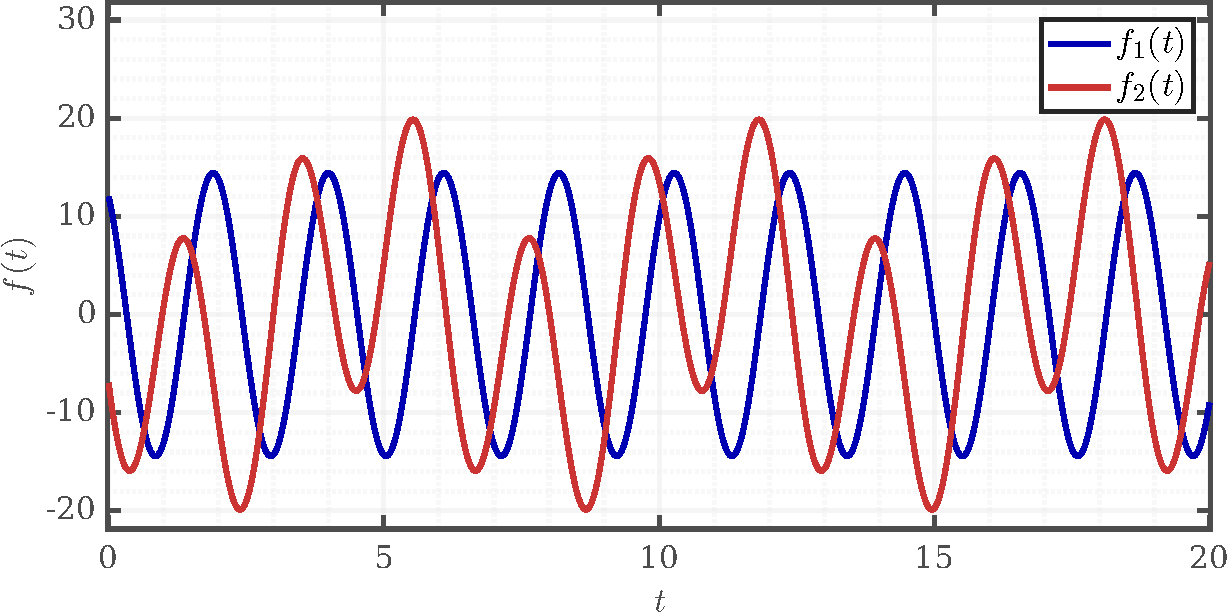
\includegraphics[width=\figwidth]{../images/task1/f_u0.pdf}
		\caption{Внешнее возмущение \(f(t)\)}
	\end{figure}
	
	\begin{figure}[H]
		\centering
		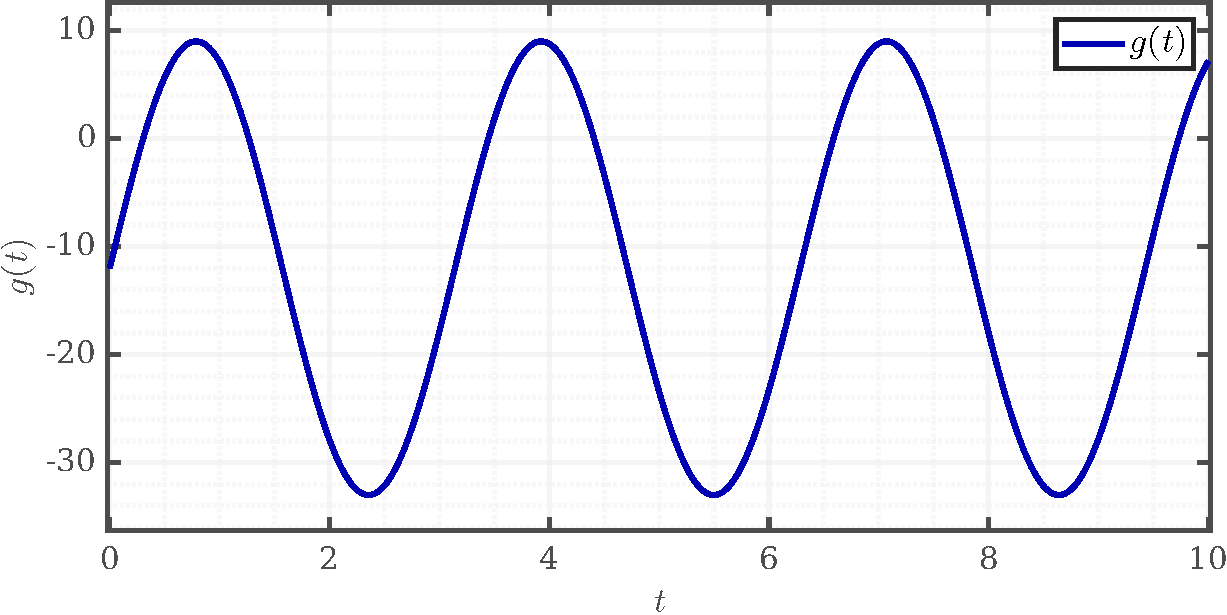
\includegraphics[width=\figwidth]{../images/task1/g_u0.pdf}
		\caption{Задающее воздействие \(g(t)\)}
	\end{figure}
	
	
	\begin{figure}[H]
		\centering
		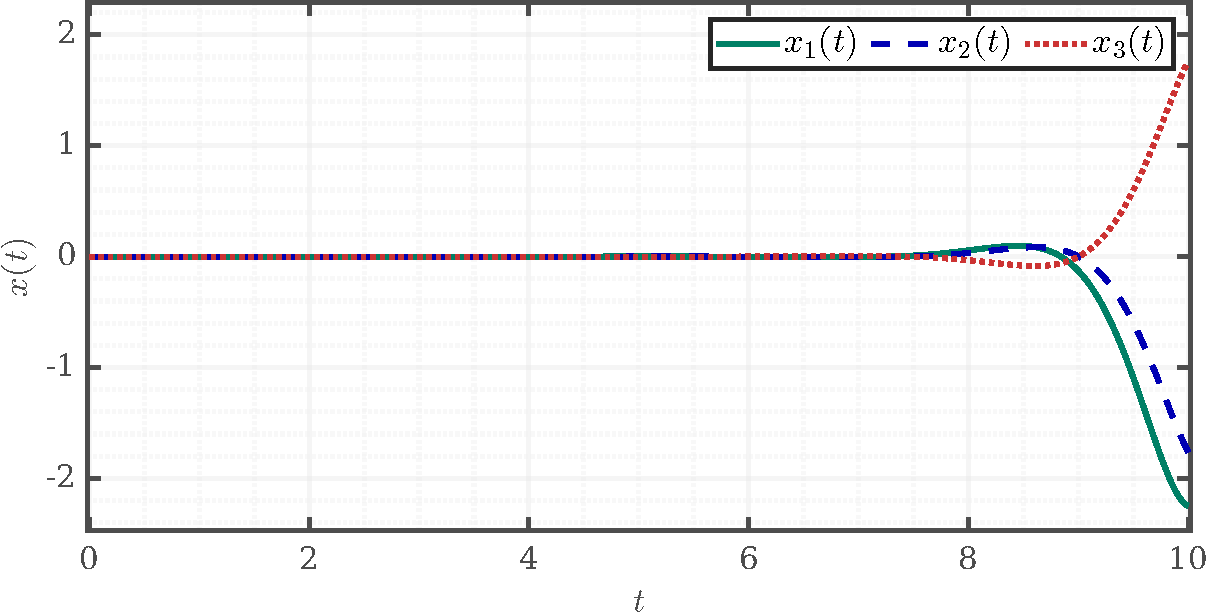
\includegraphics[width=\figwidth]{../images/task1/x_u0.pdf}
		\caption{Вектор состояния \(x(t)\)}
	\end{figure}
	
	
	\begin{figure}[H]
		\centering
		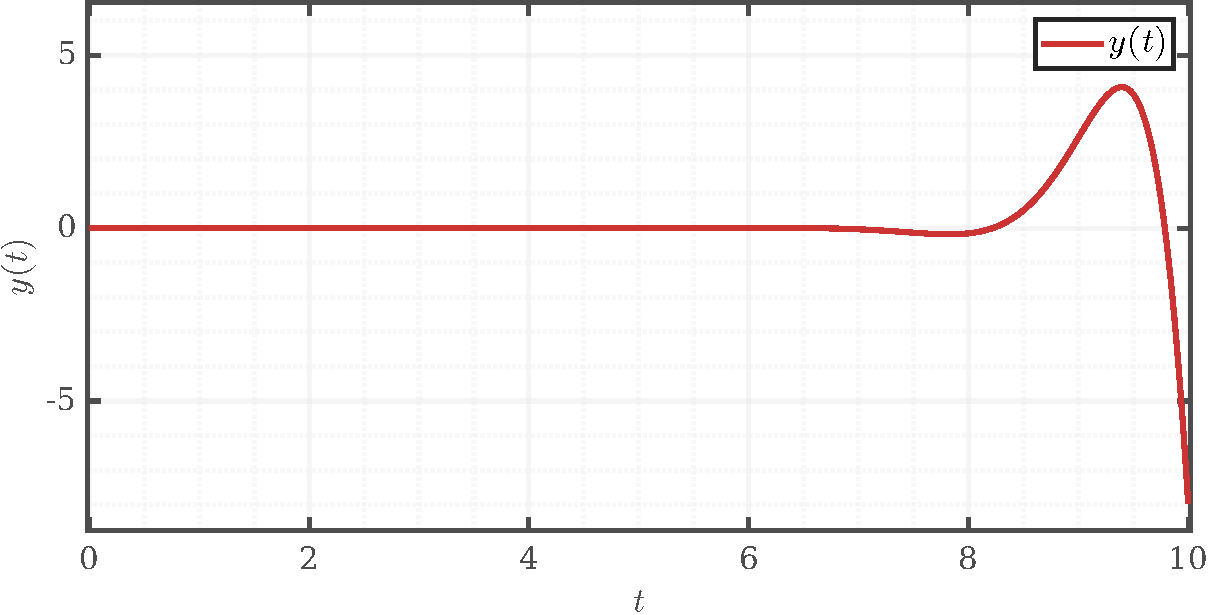
\includegraphics[width=\figwidth]{../images/task1/y_u0.pdf}
		\caption{Выход \(y(t)\)}
	\end{figure}
	
	
	
	\subsubsection{Графики компонент \(x(t)\) для замкнутых систем}
	
	Проведу моделирование системы при ее замыкании регуляторами: 
	
	\[
	u = K x \qquad
	u = K x + K_f w_f \qquad
	u = K x + K_g w_g \qquad
	u = K x + K_f w_f + K_g w_g \qquad
	\]
	
	Построю графики вектора состояния \(x(t)\).
	
	\begin{figure}[H]
		\centering
		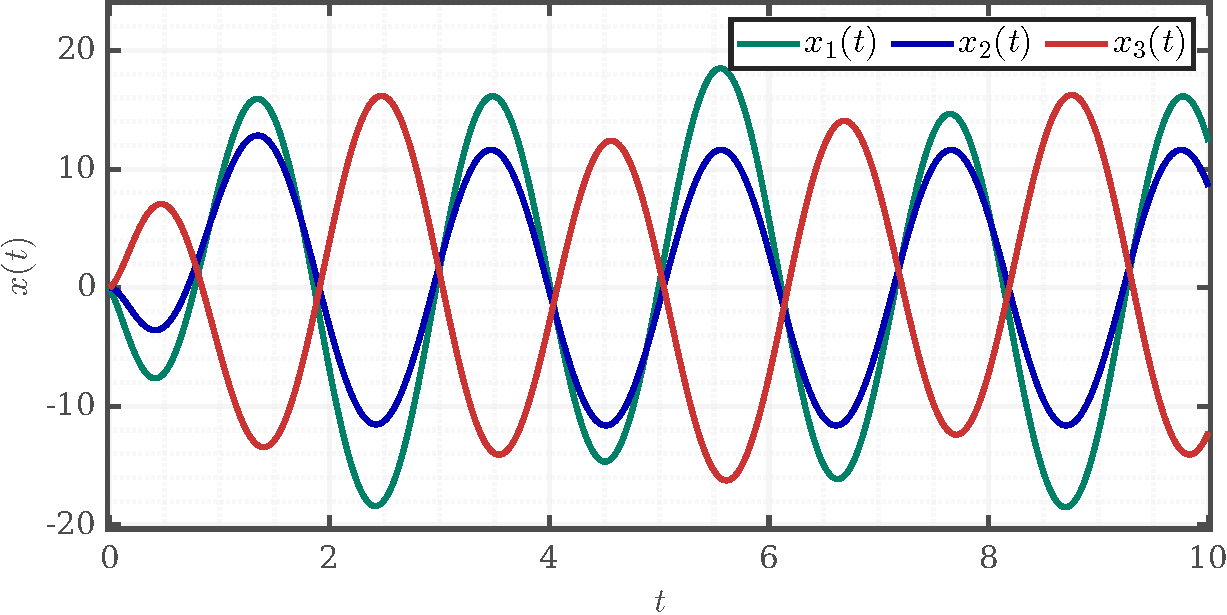
\includegraphics[width=\figwidth]{../images/task1/x_uK.pdf}
		\caption{Вектор состояния \(x(t)\) при \(u = K x\)}
	\end{figure}
	
	
	\begin{figure}[H]
		\centering
		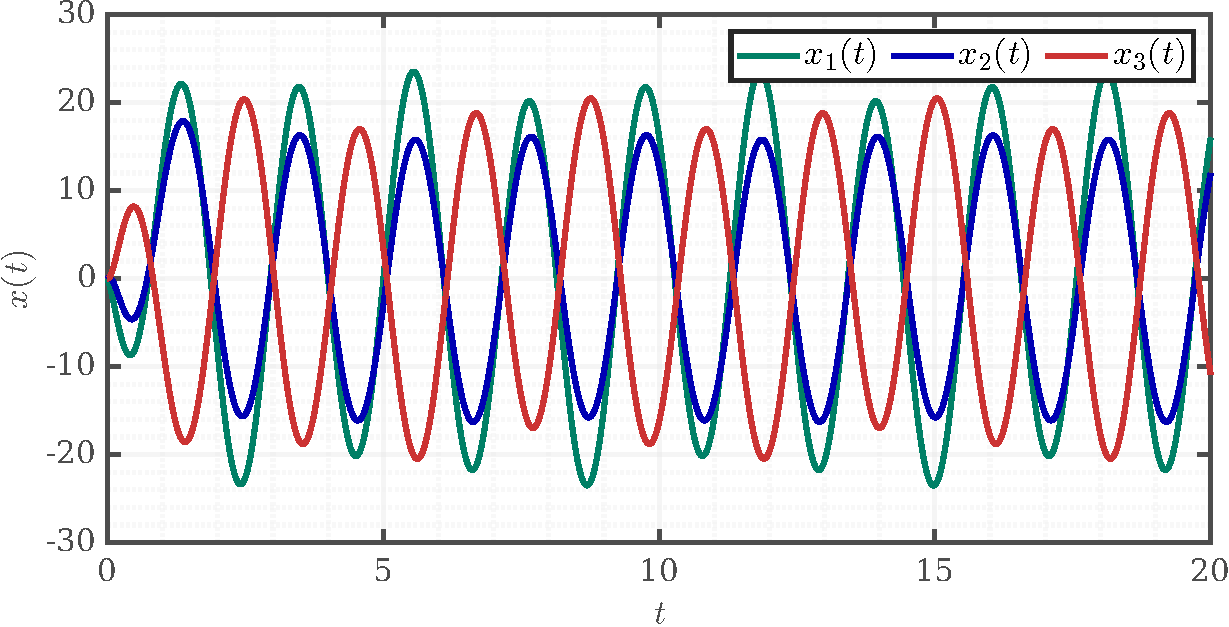
\includegraphics[width=\figwidth]{../images/task1/x_uKf.pdf}
		\caption{Вектор состояния \(x(t)\) при \(u = K x + K_f w_f\)}
	\end{figure}
	
	
	\begin{figure}[H]
		\centering
		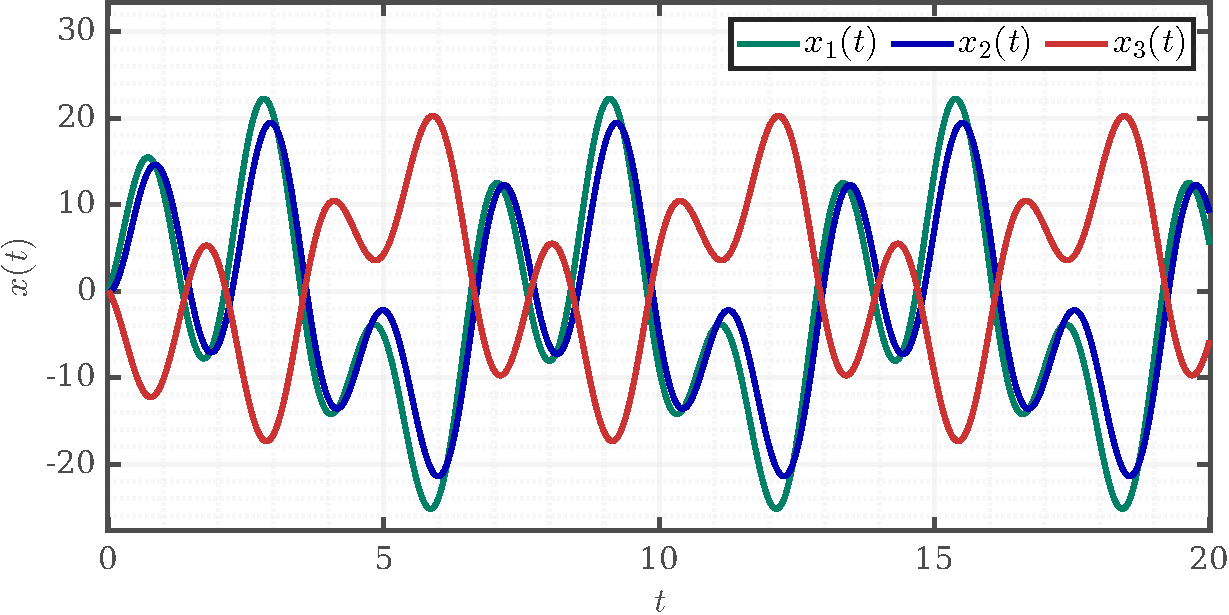
\includegraphics[width=\figwidth]{../images/task1/x_uKg.pdf}
		\caption{Вектор состояния \(x(t)\) при \(u = K x + K_g w_g\)}
	\end{figure}
	
	
	\begin{figure}[H]
		\centering
		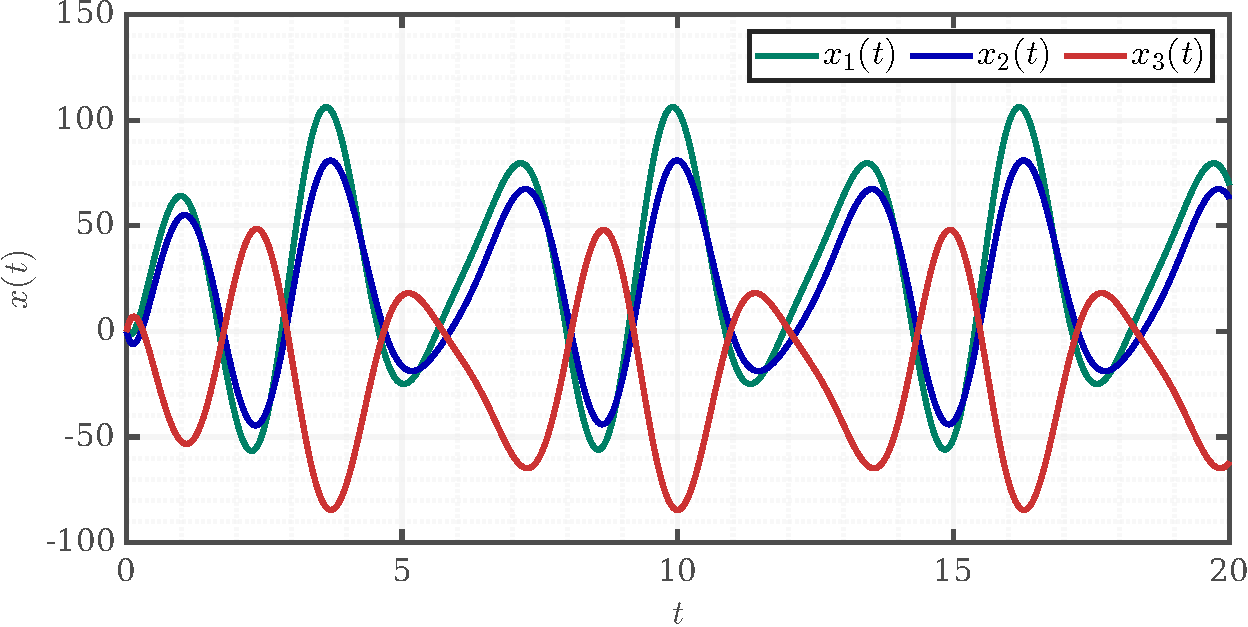
\includegraphics[width=\figwidth]{../images/task1/x_uKfg.pdf}
		\caption{Вектор состояния \(x(t)\) при \(u = K x + K_f w_f + K_g w_g\)}
	\end{figure}
	
	\subsubsection{Графики \(u(t), y(t), e(t) \) для замкнутых систем}
	
	
	Проведу моделирование системы при ее замыкании регуляторами: 
	
	\[
	u = K x \qquad
	u = K x + K_f w_f \qquad
	u = K x + K_g w_g \qquad
	u = K x + K_f w_f + K_g w_g \qquad
	\]
	
	Построю графики \(u(t)\) и \(y(t)\) на одних рисунках.
	
	\begin{figure}[H]
		\centering
		
\includegraphics[width=\figwidth]{../images/task1/u.pdf}
		\caption{Управления \(u(t)\)}
	\end{figure}
	
	
	\begin{figure}[H]
		\centering
		
\includegraphics[width=\figwidth]{../images/task1/y.pdf}
		\caption{Выходы \(y(t)\)}
	\end{figure}
	
	Проведу моделирование системы при ее замыкании регуляторами: 
	
	\[
	u = K x + K_f w_f \qquad
	u = K x + K_g w_g \qquad
	u = K x + K_f w_f + K_g w_g \qquad
	\]
	
	Построю график ошибки слежения \(e(t) = g(t) - y(t)\) на одном рисунке.
	
	\begin{figure}[H]
		\centering
		
\includegraphics[width=\figwidth]{../images/task1/e.pdf}
		\caption{Ошибки \(e(t)\)}
	\end{figure}
	
	
	\newpage
	\subsection{Вывод}
	
	Объект управления оказался неустойчивым, но стабилизируемым: неуправляемая мода с \(\lambda = -3\) является устойчивой. Обратную связь была подобрана так, чтобы замкнутая система имела три кратных полюса в \(-3\):
	
	\[
	K = \begin{bmatrix}
		-3.5 & 1 & -3.5
	\end{bmatrix} \qquad
	\sigma(A + BK) = \{-3, -3, -3\}
	\]
	
	Затем я решила матричные уравнения Франкиса-Дэвисона и получила следящую и компенсирующую компоненты:
	
	\[
	K_g = \begin{bmatrix}
		0.0703 & -0.0562 & 0.0658
	\end{bmatrix} \qquad
	K_f = \begin{bmatrix}
		-9.2262 & -2.9556 & 6.9958 & -4.9150
	\end{bmatrix}
	\]
	
	Результаты моделирования показали, что ни обратная связь по отдельности, ни пара \(K + K_f\), ни пара \(K + K_g\) не дают слежения с нулевой ошибкой. Только полный регулятор:
	
	\[
	u = Kx + K_g w_g + K_f w_f
	\]
	
	обеспечивает выполнение условия:
	
	\[
	\lim_{t \to \infty} |g(t) - y(t)| = 0
	\]
	
	Таким образом, для решения задачи слежения с компенсацией возмущений регулятор должен содержать внутреннюю модель как задающего сигнала, так и внешнего возмущения.
	
	
	\newpage \section{Слежение и компенсация по выходу}


Используя данные Задания~\ref{sec:1}, рассмотрю систему~\ref{sys}, генератор внешнего возмущения ~\ref{genF} и генератор задающего воздействия~\ref{gen}. Используя матрицы регулятора \(K\), \(K_g\) и \(K_f\), полученные в Задании 1, выполню следующие шаги:

\begin{enumerate}
	\item Построить схему моделирования системы, замкнутой регулятором:
	
	\[
	u = K \hat x + K_g \hat w_g + K_f \hat w_f
	\]
	
	обеспечивающим выполнение целевого условия:
	
	\[
	\lim_{t \to \infty} |g(t) - y(t)| = 0
	\]
	
	\item Синтезировать наблюдатель задающего воздействия. Привести выкладки и матрицу \(Q\).
	
	\item Сформировать расширенную систему и синтезировать наблюдатель расширенной размерности. Привести матрицы расширенной системы и матрицу \(L\).
	
	\item Выполнить компьютерное моделирование с нулевыми начальными условиями наблюдателей. Построить графики \(u(t)\), сравнительные графики:
	
	\[
	\begin{bmatrix} w_f(t) \\ x(t) \end{bmatrix}
	\quad \text{и} \quad
	\begin{bmatrix} \hat{w}_f(t) \\ \hat{x}(t) \end{bmatrix}
	\]
	
	график ошибки:
	
	\[
	e_f(t) = 
	\begin{bmatrix} w_f(t) \\ x(t) \end{bmatrix}
	-
	\begin{bmatrix} \hat{w}_f(t) \\ \hat{x}(t) \end{bmatrix}
	\]
	
	сравнительные графики \(w_g(t)\) и \(\hat{w}_g(t)\), график ошибки:
	
	\[
	e_g(t) = w_g(t) - \hat{w}_g(t)
	\]
	
	график выхода \(y(t)\) и график ошибки управления:
	
	\[
	e(t) = g(t) - y(t)
	\]
	
	\item Проанализировать полученные результаты в сравнении с Заданием~\ref{sec:1} и сделать выводы.
\end{enumerate}
	
	\hrule \newpage
	
	\subsection{Структурная схема системы}
	
	Построю схему моделирования системы, замкнутой регулятором, состоящим из
	наблюдателя задающего воздействия, наблюдателя расширенной размерности и закона управления:
	
	\[u = K \hat x + K_g \hat w_g + K_f \hat w_f\]
	
	обеспечивающим выполнение целевого условия:
	
	\[
	\lim_{t \to \infty} |g(t) - y(t)| = 0
	\]
	
	\begin{figure}[H]
		\centering
		
\includegraphics[width=1\textwidth]{../images/task2/model2.png}
		\caption{Схема моделирования системы, замкнутой регулятором \(u = K \hat x + K_g \hat w_g + K_f \hat w_f\)}
	\end{figure}
	\subsection{Синтез наблюдателя задающего воздействия}
	
	Для генератора задающего воздействия \eqref{gen} введу преобразование базиса:
	
	\[
	\bar{w}_g=Q_g\hat{w}_g
	\]
	И в новом базисе построю  наблюдатель в форме:
	
	\[
	\dot{\bar{w}}_g=\Gamma \bar{w}_g+Yg
	\]
	
	Пусть желаемая динамика наблюдателя будет иметь вид (учитывая, что пара \(\Gamma, Y\) наблюдаема):
	
	\[
	\Gamma=
	\begin{bmatrix}
		-5&0&0\\
		0&-6&0\\
		0&0&-7
	\end{bmatrix}
	\qquad
	Y=
	\begin{bmatrix}
		1\\7\\8
	\end{bmatrix}
	\]
	
	Матрицу \(Q\) найду из уравнения Сильвестра:
	
	\[
	Q \Gamma_g-\Gamma Q=YY_g
	\]
	
	Полученная матрица \(Q\) (листинг~\ref{lst:Q}):
	
	\[
	Q=
	\begin{bmatrix}
    0.2000  &  0.1724  & -0.0690 \\
	1.1667   & 1.0500   &-0.3500 \\
	1.1429  &  1.0566  & -0.3019 \\

	\end{bmatrix}
	\]
	
	\subsection{Синтез наблюдателя расширенной размерности}
	
	
	Рассмотрю объект управления и генератор возмущения в одной расширенной системе:
	
	\begin{align*}
		&\begin{cases}
			\dot w_f = \Gamma_f w_f \\
			\dot x = A x + B u + B_f Y_f w_f \\
			y = C x + D u + D_f Y_f w_f
		\end{cases} \\
		&\begin{cases}
			x_f = \begin{bmatrix}
				w_f \\ x \\
			\end{bmatrix} \\
			\dot x_f = \bar{A} x_f + \bar B u \\
			y = \bar C x_f + D u
		\end{cases}
	\end{align*}
	
	Матрицы \(\bar A, \bar B, \bar C\):
	
	\[
	\bar{A}=
	\begin{bmatrix}
		\Gamma_f&0\\
		B_fY_f&A
	\end{bmatrix} \qquad
	\bar B = \begin{bmatrix}
		0 \\ B
	\end{bmatrix} 
	\qquad
		\bar C = \begin{bmatrix}
		D_f Y_f & C
	\end{bmatrix}
	\]
	
	Наблюдатель расширенной размерности имеет вид:
	\[
	\begin{cases}
		\dot{\hat{x}}_f=\bar{A}\hat{x}_f+(\bar{B}+LD)u+L(\hat{y}-y)\\
		\hat{y}=\bar{C}\hat{x}_f
	\end{cases}
	\]
	
	Синтезирую матрицу наблюдателя \(L\). Пусть:
	
	\[
	\sigma(\bar A + L \bar C) = \{-3\pm0.5\mathrm{j},\; -3.2\pm1\mathrm{j},\; -3.5\pm1.5\mathrm{j},\; -5\}
	\]
	
	Тогда матрица наблюдателя имеет вид (листинг~\ref{lst:L}):
	
	\[
	L = \begin{bmatrix}
		   13.1597 \\
		7.3996 \\
		28.5143 \\
		13.9307 \\
		-366.5229 \\
		-229.7677 \\
		231.3229 \\
	\end{bmatrix}
	\]
	
	Проверка собственных чисел \(\bar A + L \bar C\) показала корректность расчета.
	
	
	\subsection{Моделирование}
	
	Проведу моделирование системы, выставив нулевые начальные условия наблюдателей. Построю графики управления, выхода и ошибки слежения:
	
	\begin{figure}[H]
		\centering
		
\includegraphics[width=\figwidth]{../images/task2/u.pdf}
		\caption{Управление \(u(t) = K\hat{x} + K_g \hat{w}_g + K_f \hat{w}_f\)}
	\end{figure}
	
	\begin{figure}[H]
		\centering
		
\includegraphics[width=\figwidth]{../images/task2/y.pdf}
		\caption{Выход \(y(t)\)}
	\end{figure}
	
	
	\begin{figure}[H]
		\centering
		
\includegraphics[width=\figwidth]{../images/task2/e.pdf}
		\caption{Ошибка \(e(t) = g(t) - y(t)\)}
	\end{figure}
	
Сравню реальные и оценённые состояния

\begin{figure}[H]
	\centering
	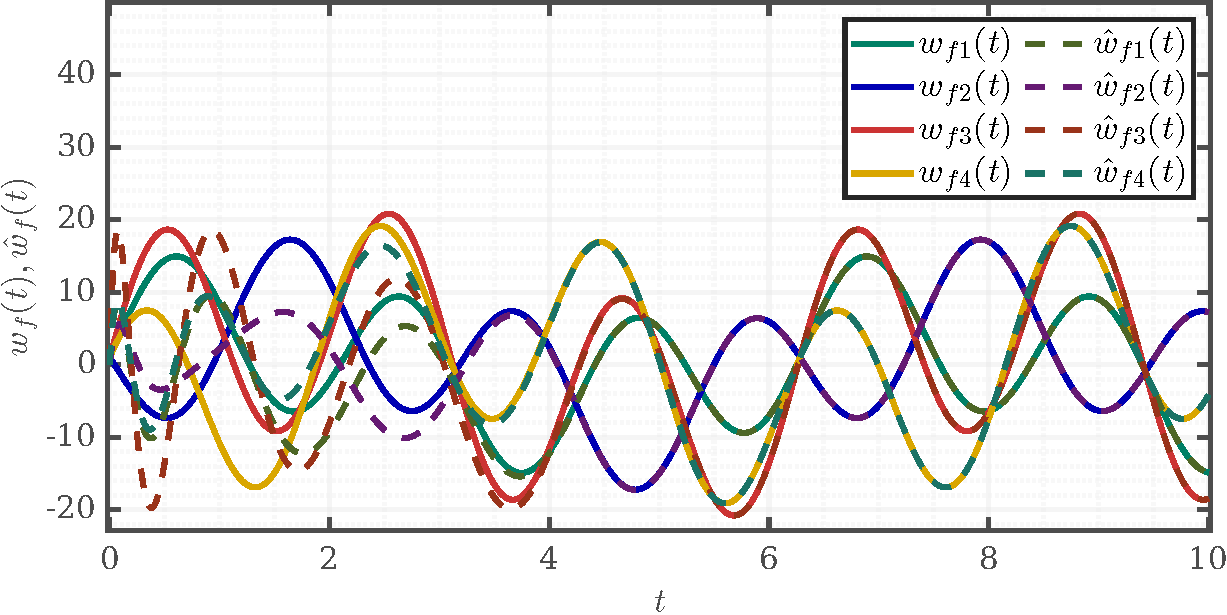
\includegraphics[width=\figwidth]{../images/task2/wf.pdf}
	\caption{Сравнение \(w_f(t)\) и \(\hat{w}_f(t)\)}
\end{figure}

\begin{figure}[H]
	\centering
	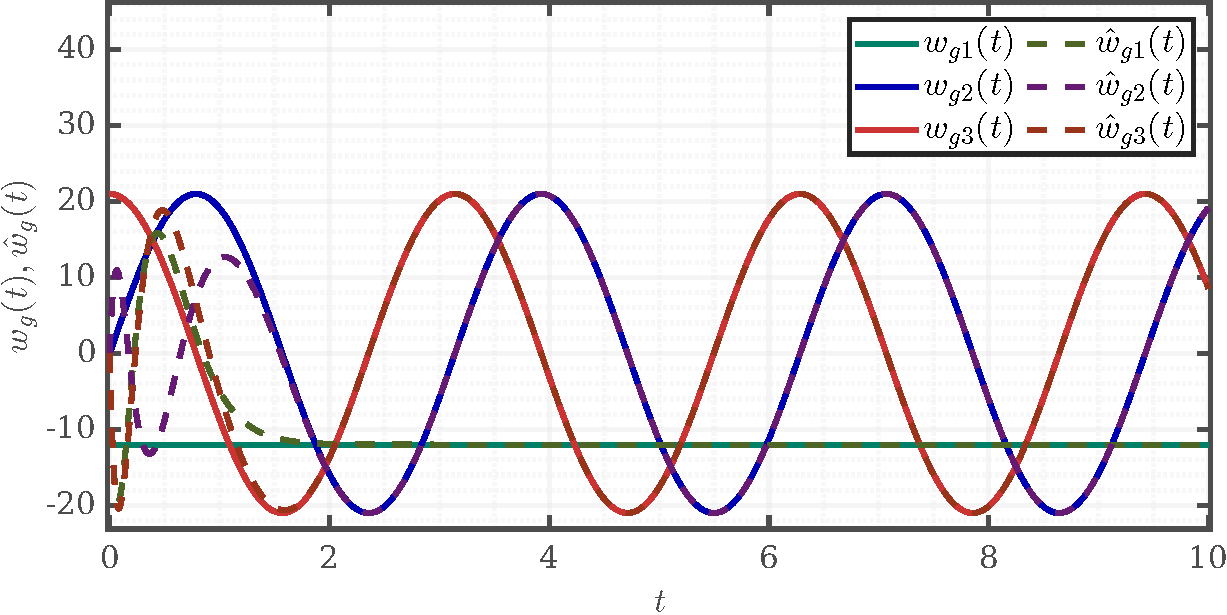
\includegraphics[width=\figwidth]{../images/task2/wg.pdf}
	\caption{Сравнение \(w_g(t)\) и \(\hat{w}_g(t)\)}
\end{figure}

\begin{figure}[H]
	\centering
	
\includegraphics[width=\figwidth]{../images/task2/x.pdf}
	\caption{Сравнение \(x(t)\) и \(\hat{x}(t)\)}
\end{figure}

Построю графики ошибок наблюдения:

\[
e_{wf}(t) = w_f(t) - \hat{w}_f(t)
\]

\[
e_x(t) = x(t) - \hat{x}(t)
\]

\[
e_g(t) = w_g(t) - \hat{w}_g(t)
\]

\begin{figure}[H]
	\centering
	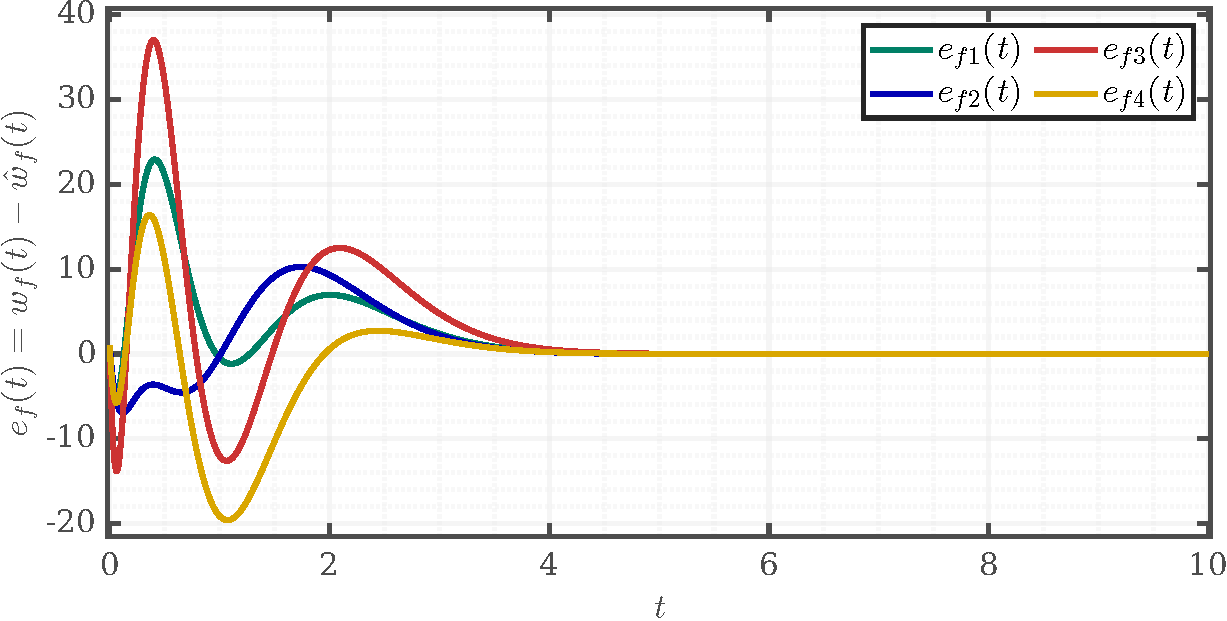
\includegraphics[width=\figwidth]{../images/task2/ef.pdf}
	\caption{Ошибка восстановления \(w_f(t)\)}
\end{figure}

\begin{figure}[H]
	\centering
	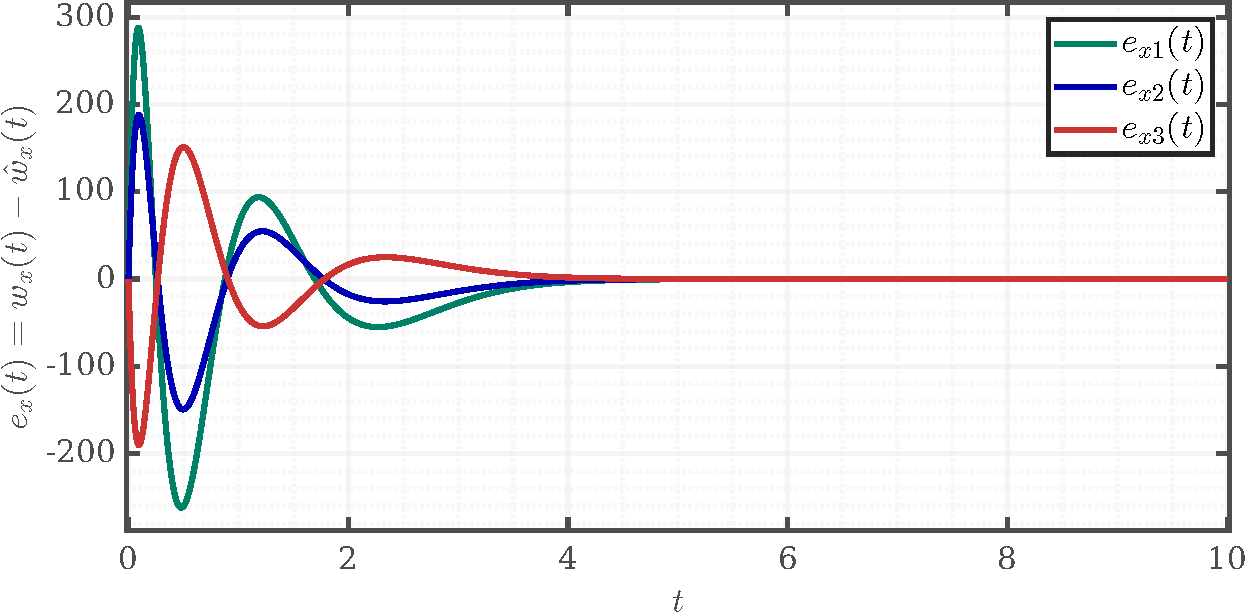
\includegraphics[width=\figwidth]{../images/task2/ex.pdf}
	\caption{Ошибка восстановления \(x(t)\)}
\end{figure}

\begin{figure}[H]
	\centering
	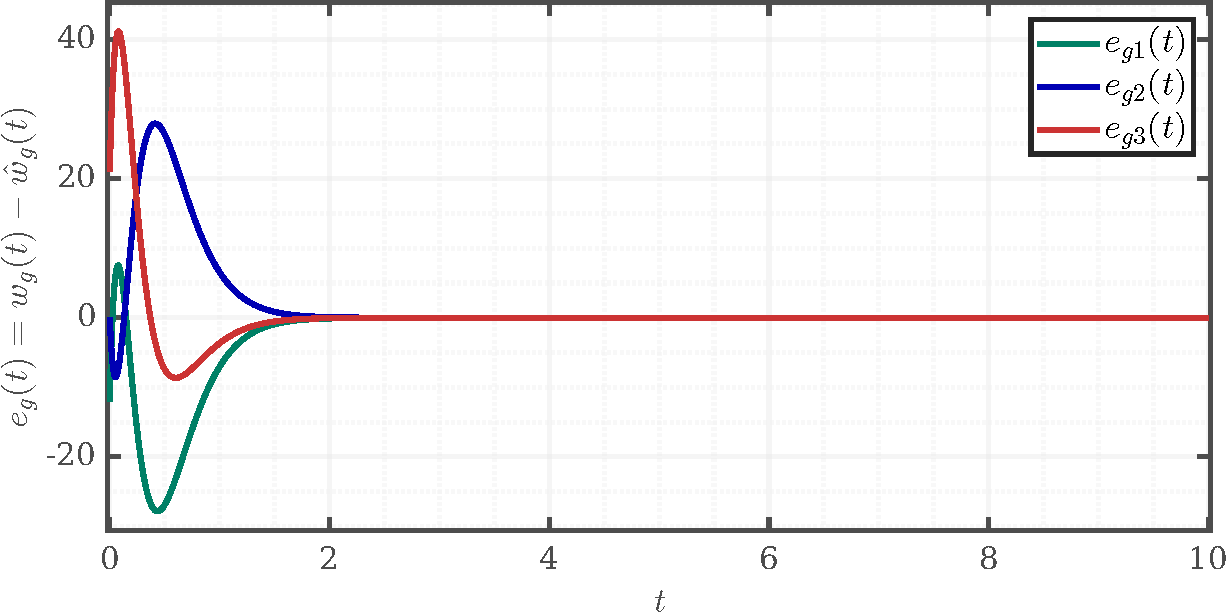
\includegraphics[width=\figwidth]{../images/task2/eg.pdf}
	\caption{Ошибка наблюдателя задающего воздействия \(e_g(t) = w_g(t) - \hat{w}_g(t)\)}
\end{figure}
	
	
	\newpage
	
	\subsection{Вывод}
	
	Во втором задании я синтезировала наблюдатель задающего воздействия и наблюдатель расширенной размерности. Полученные матрицы:
	
	\[
	Q =
	\begin{bmatrix}
		0.2000 & 0.1724 & -0.0690 \\
		1.1667 & 1.0500 & -0.3500 \\
		1.1429 & 1.0566 & -0.3019
	\end{bmatrix} \qquad
	L =
	\begin{bmatrix}
		13.1597 \\
		7.3996 \\
		28.5143 \\
		13.9307 \\
		-366.5229 \\
		-229.7677 \\
		231.3229
	\end{bmatrix}
	\]
	
	Моделирование показало, что ошибки наблюдения сходятся к нулю, выход отслеживает задающий сигнал.
	
	По сравнению с предыдущим заданием, где все переменные состояния были доступны, переходный процесс здесь получился более длительным. Это объясняется наличием начальных ошибок наблюдателей: оценки сходятся к истинным значениям не мгновенно, что влияет на качество управления на начальном участке.
	
	Тем не менее, в установившемся режиме регулятор с наблюдателями обеспечивает слежение
	
	\[
	\lim_{t \to \infty} |g(t) - y(t)| = 0
	\]
	
Предложенная структура позволяет решить задачу даже при недоступности переменных состояния для измерения.
	
	
	
	
	
	
	
	
	
	
	
	
	
	\newpage
	\section{Приложение}
	
\subsection*{Задание 1}

\begin{lstlisting}[caption={Инициализация}, language=matlab]
A = [8 1 11; 4 0 4; -4 -3 -7];
B = [-1; -3; 3];
C = [-2 0 -3];
D = 15;
B_f = [1, -1; 0, 0; -1, 0];
D_f = [0 3];
wf0 = [1; 1; 1; 1];
G_f = [35 10 -28 17; -22 -7 18 -12; 56 17 -45 27; 34 12 -28 17];
Y_f = [12 -6; 4 -2; -10 4; 6 -3].';
G_g = [0 0 0; 0 0 2; 0 -2 0];
Y_g = [1, 1, 0];
wg0 = [-12; 0; 21];
x0 = [0; 0; 0];
K = [-3.5 1 -3.5];
\end{lstlisting}

\begin{lstlisting}[caption={Спектр \(\Gamma_f\)}, label={lst:eig1}, language=matlab]
eig(G_f)
\end{lstlisting}


\begin{lstlisting}[caption={Поиск вещественной Жордановой формы}, label={lst:jordan1}]
[P, J] = jordan(sym(A)); P = double(P); J = double(J);
[P_real, J_real] = cdf2rdf(P, J)
B_tilde = inv(P_real) * B
\end{lstlisting}

\begin{lstlisting}[caption={Решение уравнения Сильвестра}, label={lst:silv1}]
A2 = J_real(2:3, 2:3);
B2 = B_tilde(2:3);
G = [-3 1; 0 -3];
Y = [1 2];

P = lyap(A2, -G, -B2*Y)
K2 = -Y * P^-1
\end{lstlisting}

\begin{lstlisting}[caption={Перевод \(\hat K_c\) в исходный базис}, label={lst:origK11}]
K = [0 K2] * P_real^-1
\end{lstlisting}

\begin{lstlisting}[caption={Собственные числа матрицы замкнутой системы}, label={lst:eigA}]
z = A + B*K
eig(z)
\end{lstlisting}

\begin{lstlisting}[caption={Проверка разрешимости}, label={lst:checkkg}]
for lam = eig(G_g)'
M = [A+B*K-lam*eye(n), B; C+D*K, D];
fprintf('rank = %d (need %d) for lam = %.2f%+.2fi\n', rank(M), n+m, real(lam), imag(lam));
end
\end{lstlisting}

\begin{lstlisting}[caption={Синтез \(K_g\)}, label={lst:solvekg}]
r = size(G_g,1);
I = @(x) eye(x);
M11 = kron(G_g', I(n)) - kron(I(r), A);
M12 = -kron(I(r), B);
M21 = kron(I(r), C);
M22 = D * I(r);
sol = [M11, M12; M21, M22] \ [zeros(n*r,1); Y_g'];
X_g = reshape(sol(1:n*r), n, r);
U_g = sol(n*r+1:end)';
K_g = U_g - K*X_g;
\end{lstlisting}

\begin{lstlisting}[caption={Проверка разрешимости}, label={lst:checkkf}]
for lam = eig(G_f)'
M = [A+B*K-lam*eye(n), B; C+D*K, D];
fprintf('rank = %d (need %d) for lam = %.2f%+.2fi\n', rank(M), n+m, real(lam), imag(lam));
end
\end{lstlisting}

\begin{lstlisting}[caption={Синтез \(K_f\)}, label={lst:solvekf}]
p = size(G_f,1);
M11 = kron(G_f', I(n)) - kron(I(p), A);
M12 = -kron(I(p), B);
M21 = kron(I(p), C);
M22 = D * I(p);
sol = [M11, M12; M21, M22] \ [reshape(B_f*Y_f, [], 1); (-D_f*Y_f)'];
X_f = reshape(sol(1:n*p), n, p);
U_f = sol(n*p+1:end)';
K_f = U_f - K*X_f;

\end{lstlisting}

\newpage
\subsection*{Задание 2}

\begin{lstlisting}[caption={Инициализация}, language=matlab]
A = [8 1 11; 4 0 4; -4 -3 -7];
B = [-1; -3; 3];
C = [-2 0 -3];
D = 15;
B_f = [1, -1; 0, 0; -1, 0];
D_f = [0 3];
wf0 = [1; 1; 1; 1];
G_f = [35 10 -28 17; -22 -7 18 -12; 56 17 -45 27; 34 12 -28 17];
Y_f = [12 -6; 4 -2; -10 4; 6 -3].';
G_g = [0 0 0; 0 0 2; 0 -2 0];
Y_g = [1, 1, 0];
wg0 = [-12; 0; 21];
x0 = [0; 0; 0];
K = [-3.5 1 -3.5];
K_f = [-9.2262 -2.9556  6.9958 -4.9150]; 
K_g = [0.0703 -0.0562  0.0658]; 
G = [-5 0 0; 0 -6 0; 0 0 -7];
Y = [1; 7; 8];
\end{lstlisting}

\begin{lstlisting}[caption={Поиск \(Q\) и \(Q_{inv}\)}, label={lst:Q}, language=matlab]
Q = lyap(G_g', -G, -(Y*Y_g)')';
Q_inv = inv(Q);
\end{lstlisting}
	
\begin{lstlisting}[caption={Поиск \(L\)}, label={lst:L}, language=matlab]
poles = [-3.0+0.5i, -3.0-0.5i, -3.2+1.0i, -3.2-1.0i, -3.5+1.5i, -3.5-1.5i, -5];
L = place(A_bar', -C_bar', poles)';
\end{lstlisting}
	
\end{document}